\documentclass[border=10pt]{standalone}
\usepackage{pgfplots}
\pgfplotsset{width=15cm,compat=1.8}
\begin{document}
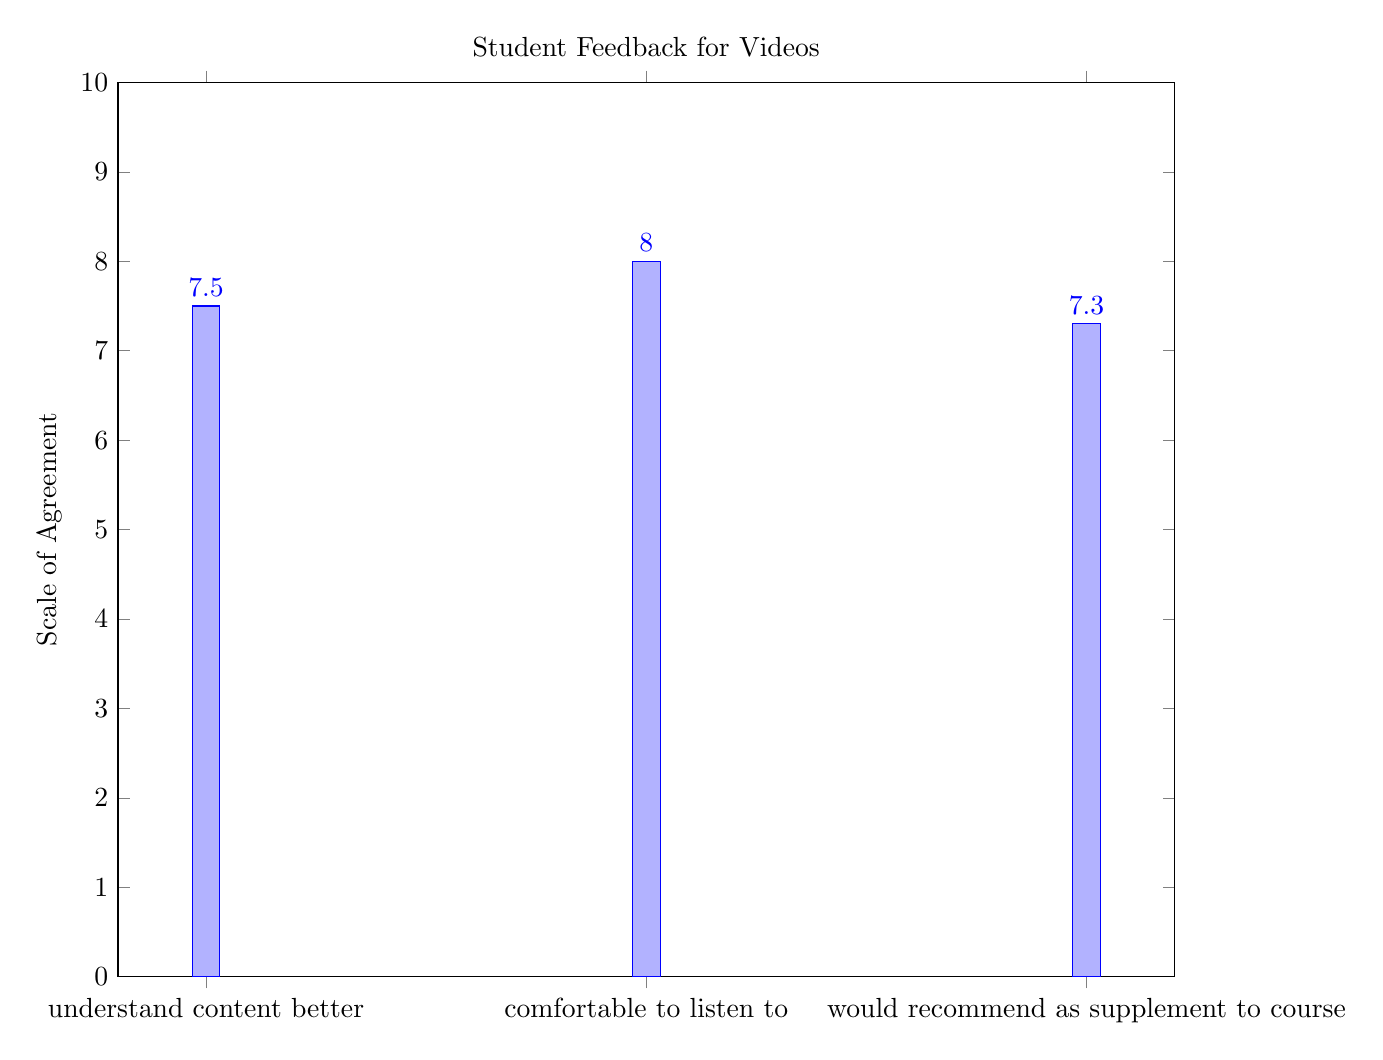
\begin{tikzpicture}
\begin{axis}[
    title = {Student Feedback for Videos},
    ybar,
    ymin = 0,
	ymax = 10,
	%enlargelimits=0.2,
    legend style={at={(0.5,-0.15)},
      anchor=north,legend columns=-1},
    ylabel={Scale of Agreement},
	symbolic x coords={understand content better, comfortable to listen to, would recommend as supplement to course},
    xtick=data,
    nodes near coords,
    nodes near coords align={vertical},
    ]
	\addplot coordinates {(understand content better, 7.5) (comfortable to listen to, 8.0) (would recommend as supplement to course, 7.3)};

\end{axis}
Figure denotes the average scores of 38 responses to each statement
\end{tikzpicture}
\end{document}
